\subsection{Testing Directory traversal/file include - OTG-AUTHZ-001}
\subsubsection{BANK-APP}
\begin{longtable}[l]{ p{2.3cm} | p{.79\linewidth} }\hline
    & \textbf{BANK-APP}
    \hfill CVSS Score: 7.5 \progressbar[filledcolor=red]{0.75}
    \\ \hline
    \textbf{Observation} &
    	Directory indexing is activated for
    	\begin{itemize}
    		\item \code{http://IP\_ADDRESS/secure-coding/}
    		\item \code{http://IP\_ADDRESS/secure-coding/app/}
    		\item \code{http://IP\_ADDRESS/secure-coding/public/}
    	\end{itemize}
    	Directly accessing the PHP files in the \code{app} folder is not permitted. The C program can be downloaded in the \code{app} folder. Futhermore, in the \code{secure-coding} folder a database dump can be seen including entries for an employee and client account. The \code{public} folder shows all possible URLs. \\
    \textbf{Discovery} & The command \code{nikto -h http://IP\_ADDRESS/secure-coding} lists information about the server and its vulnerabilities. It also lists paths for which directory indexing is activated. \\
    \textbf{Likelihood} & Accessing the directory listing does not require any extra skill. It can be directly accessed through the browser. \\
    \textbf{Impact} & Since there is a database dump with entries for an employee and a client account, a hacker only needs to bruteforce the password. Moreover, it is easier to inject SQL, if the database structure is known. With the directory listing in the \code{public} folder a hacker also knows all possible URLs. \\
    \textbf{Recommen\-dations} & Disable directory listing for hiding sensitive information. \\ \hline
    \textbf{CVSS} &
        \begin{tabular}[t]{@{}l | l}
            Attack Vector           & \textcolor{red}{Network} \\
            Attack Complexity       & \textcolor{red}{Low} \\
            Privileges Required     & \textcolor{red}{None} \\
            User Interaction        & \textcolor{red}{None} \\
            Scope                   & \textcolor{Green}{Unchanged} \\
            Confidentiality Impact  & \textcolor{red}{High} \\
            Integrity Impact        & \textcolor{Green}{None} \\
            Availability Impact     & \textcolor{Green}{None}
        \end{tabular}
    \\ \hline
\end{longtable}

\subsubsection{SecureBank}
\begin{longtable}[l]{ p{2.3cm} | p{.79\linewidth} }\hline
    & \textbf{SecureBank}
    \hfill CVSS Score: 5.3 \progressbar[filledcolor=BurntOrange]{0.53}
    \\ \hline
    \textbf{Observation} &
    	Directory indexing is activated for
    	\begin{itemize}
    		\item \code{http://IP\_ADDRESS/tmp/}
    		\item \code{http://IP\_ADDRESS/Vendor/}
    		\item \code{http://IP\_ADDRESS/Style/}
    		\item \code{http://IP\_ADDRESS/Script/}
    	\end{itemize}
    	The \code{tmp} folder lists some old text files for making transactions. The other folders contains stylesheets and JavaScript files. \\
    \textbf{Discovery} & The command \code{nikto -h http://IP\_ADDRESS} lists information about the server and its vulnerabilities. It also lists paths for which directory indexing is activated. \\
    \textbf{Likelihood} & Accessing the directory listing does not require any extra skill. It can be directly accessed through the browser. The challenge in this case is to find out the URLs for which directory indexing is activated. \\
    \textbf{Impact} & Although a hacker can access some directory listing, there are no confidential files, which he could access. \\
    \textbf{Recommen\-dations} & Disable directory listing for hiding sensitive information. \\ \hline
    \textbf{CVSS} &
        \begin{tabular}[t]{@{}l | l}
            Attack Vector           & \textcolor{red}{Network} \\
            Attack Complexity       & \textcolor{red}{Low} \\
            Privileges Required     & \textcolor{red}{None} \\
            User Interaction        & \textcolor{red}{None} \\
            Scope                   & \textcolor{Green}{Unchanged} \\
            Confidentiality Impact  & \textcolor{BurntOrange}{Low} \\
            Integrity Impact        & \textcolor{Green}{None} \\
            Availability Impact     & \textcolor{Green}{None}
        \end{tabular}
    \\ \hline
\end{longtable}

\subsubsection{Comparison}
Although both bank applications have (partly) directory indexing enabled, the vulnerability for BANK-APP is much higher since a hacker can access confidential information. Downloading the database dump file and looking at it in a text editor it can be seen there are three accounts. Figure~\ref{fig:db_dump} shows the SQL for the \code{users} table. Aside from the e-mails used for the accounts it is also visible that the accounts probably all use the same password since the hash is the same for all of them. Furthermore, for the employee and client account there are transaction codes in the dump file.

\begin{figure}[ht]
	\centering
	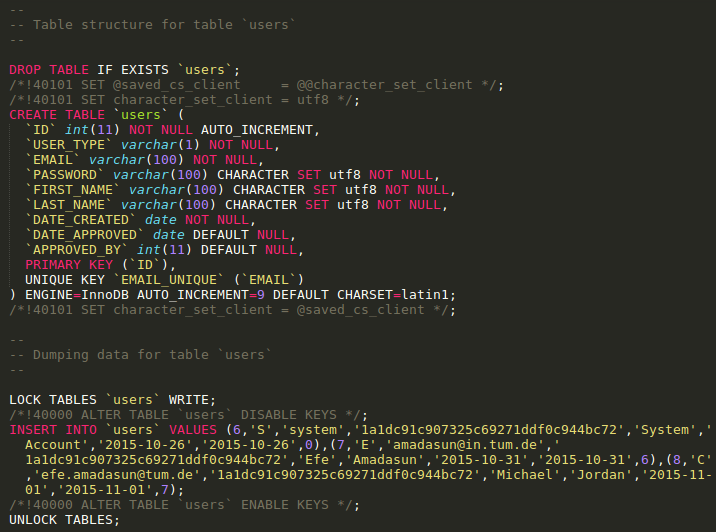
\includegraphics[width=.8\linewidth]{figures/OTG-AUTHZ-001.png}
	\caption{Database dump file of BANK-APP with account information}
	\label{fig:db_dump}
\end{figure}

\clearpage